\documentclass{beamer}
\usepackage[utf8]{inputenc}
\usepackage{caption}
\usepackage{subcaption}

\title{Strategies for computing the scalar self-force on a Schwarzschild background}
\author{Steven Dorsher}
\institute{Louisiana State University}
\date{September 26, 2017}

\begin{document}
\frame{\titlepage}


\begin{frame}
  \frametitle{Gravitational Waves}
  \begin{figure}
    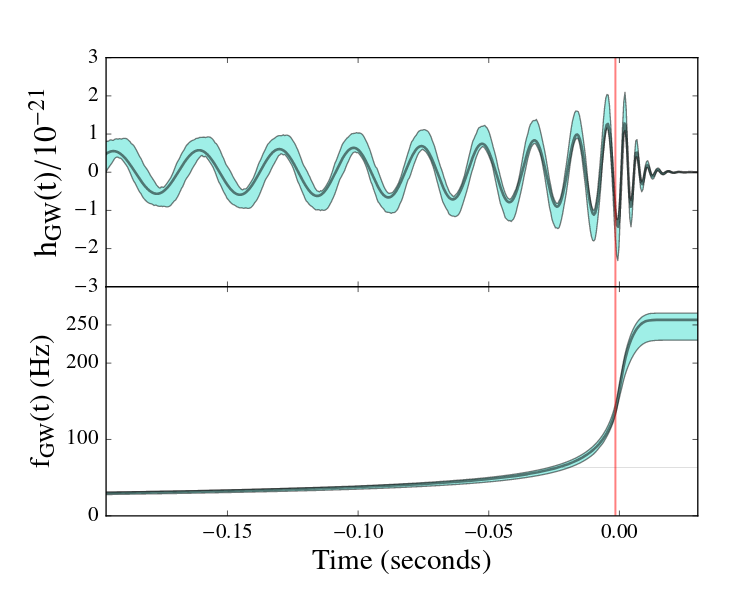
\includegraphics[width=3.0in]{LIGOGRtest.png}
    \caption{LIGO detection, September 14, 2015. General relativity was tested by comparing inpsiral with merger/ringdown phases.}
  \end{figure}
\end{frame}




\begin{frame}
  \frametitle{Extreme Mass Ratio Inspirals}
  \begin{figure}
    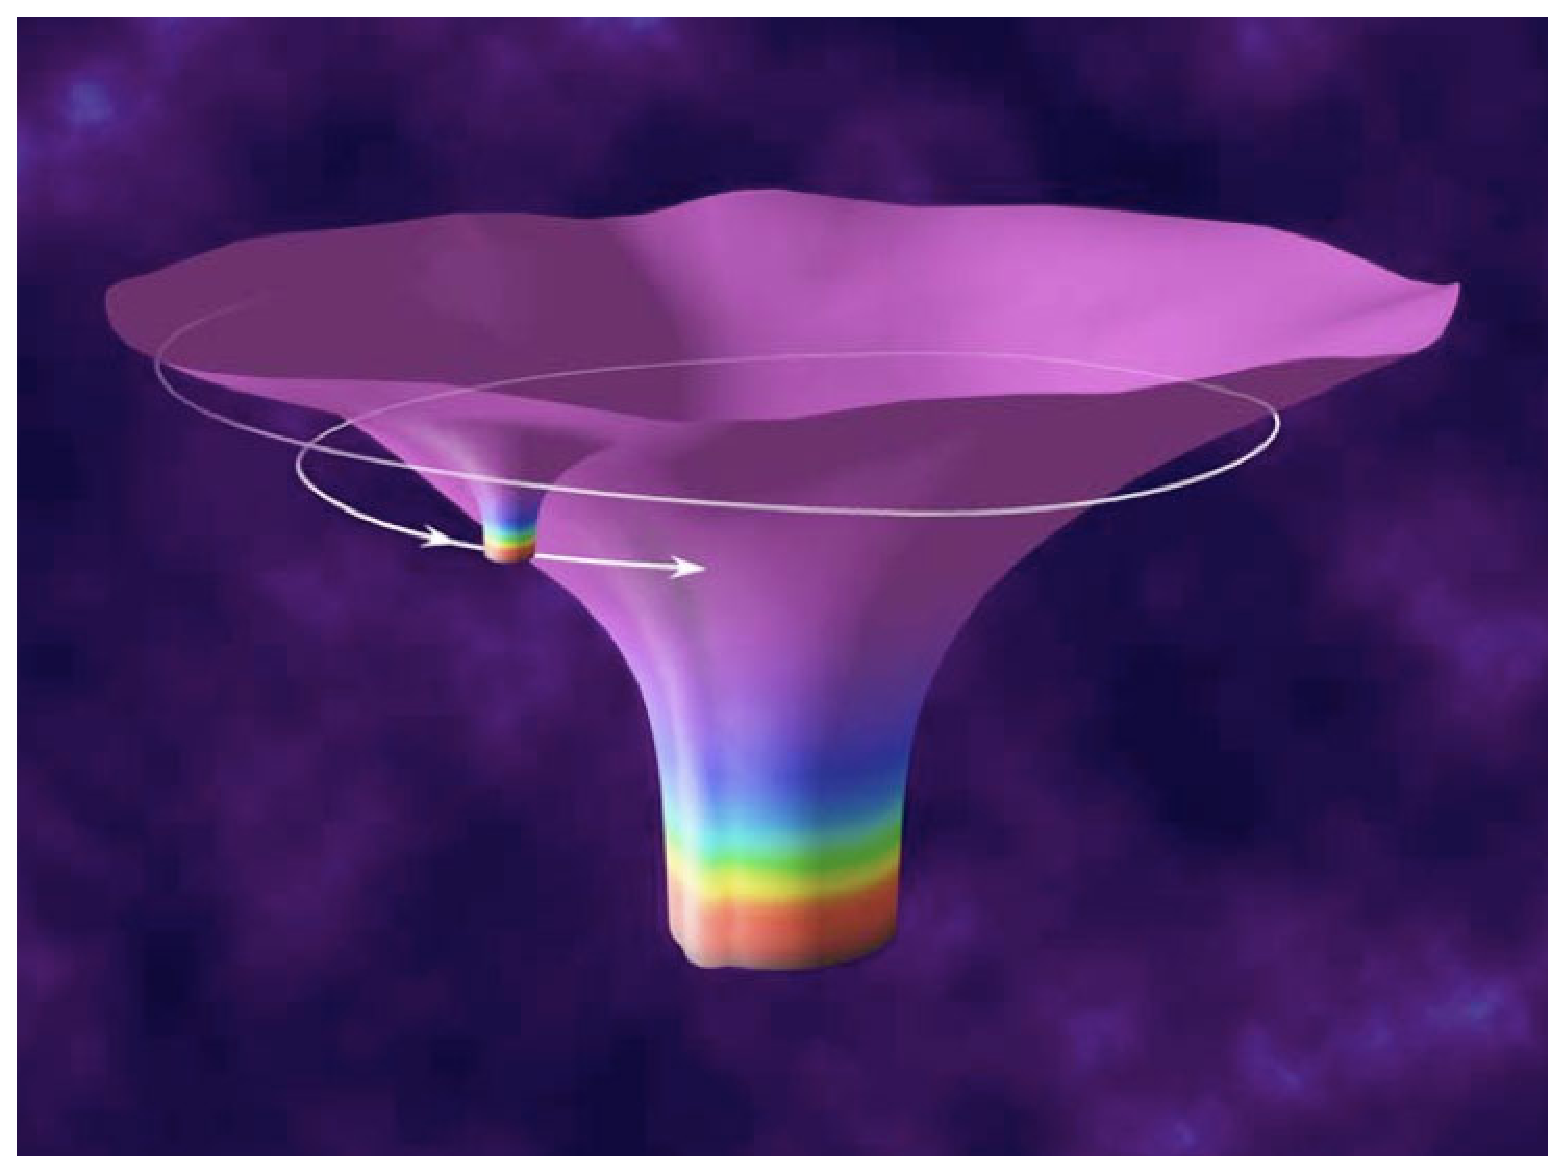
\includegraphics[width=4.0in]{EMRI}
    \citation{Extreme Mass Ratio Inspiral, $\mu=m/M\sim 10^{-4}$ to $10^{-6}$, Artist's rendition, Wikipedia}
  \end{figure}
\end{frame}

\begin{frame}
  \frametitle{Laser Interferometer Space Antenna}
  \begin{figure}
    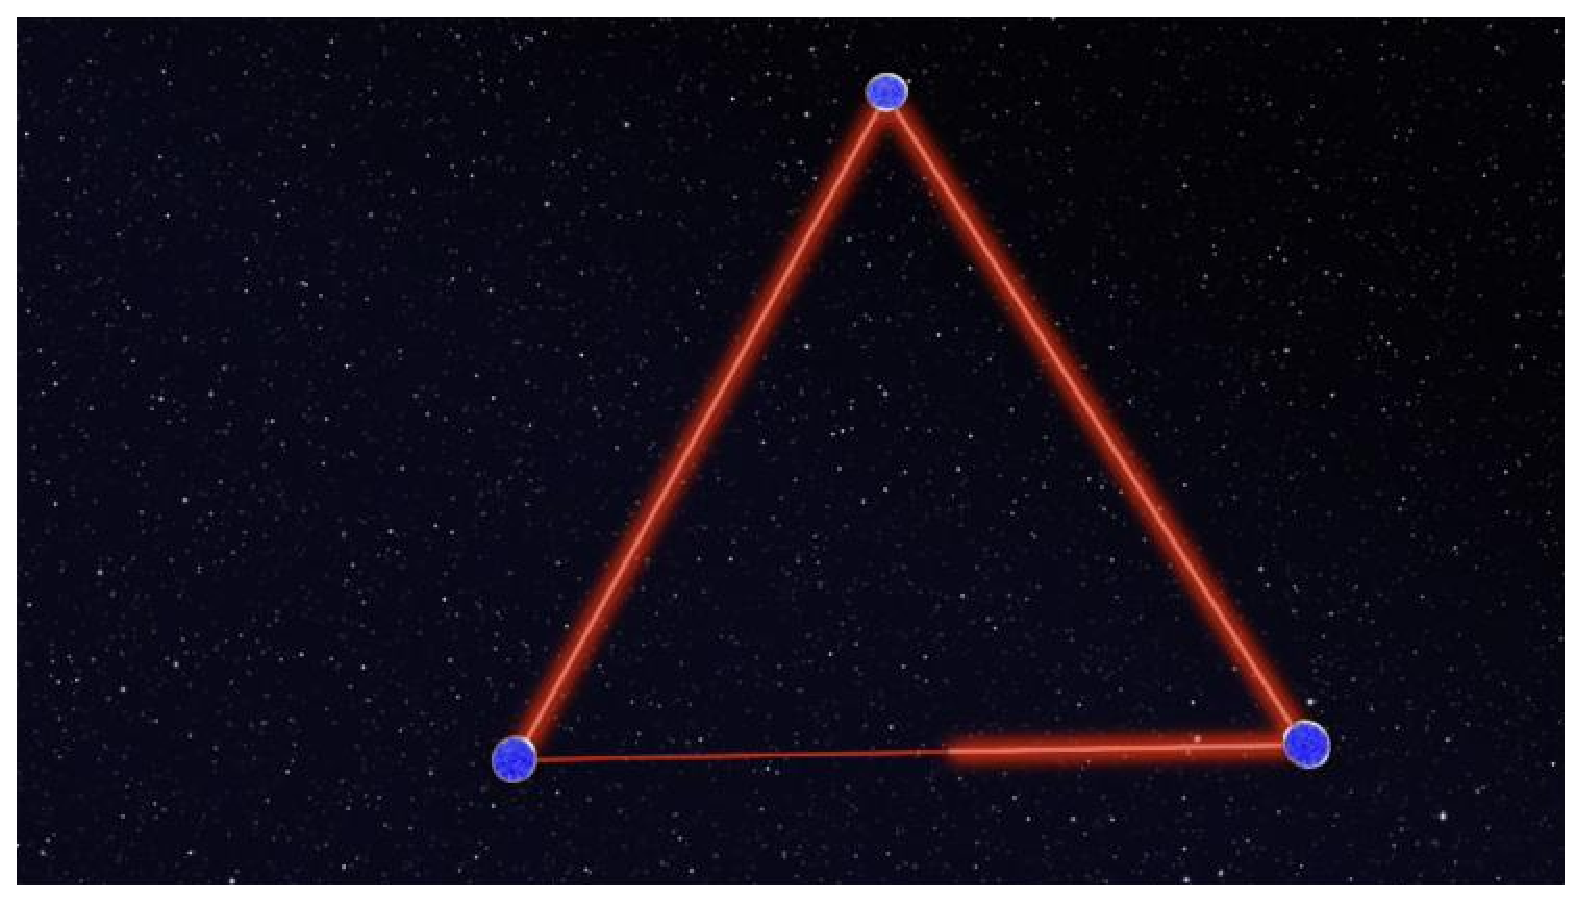
\includegraphics[width=4.0in]{eLISA}
    \caption{Laser Interferometer Space Antenna, which will operate around launches in early 2030's, ESA-NASA partnership, will detect EMRI's}
  \end{figure}
\end{frame}



\begin{frame}
  \frametitle{Toward LISA EMRI templates}
  \begin{itemize}
  \item Generating LISA EMRI templates require evolving $10^6$ orbits with precision on the order of $\delta P/P\sim 10^{-6}$ {\em Danzmann, Karsten. LISA: A proposal in response to the ESA call for L3 mission concepts (2017)}
  \item For EMRI's, the self-force approximation is used in the limit where the mass ratio is large ($10^4$ to $10^6$)
  \item EMRI's have an orbital evolution timescale that scales as $M/\mu$, and a period that scales as $M$. These two widely different timescales necessitate a different numerical approach than numerical relativity.
  \item Self-force prescribes a perturbative approximation in the mass ratio. 
  \end{itemize}
\end{frame}

%\begin{frame}
%  \frametitle{Self-force in a classical atom}
%  \begin{itemize}
%  \item Consider a classical atom without quantization (not even a Bohr atom)
%  \item The electron orbits the nucleus
%  \item It radiates energy because it is accelerated
%  \item Because it radiates energy, it becomes more tightly bound
%  \item The electron spirals inward due to the interaction of the particle with its own field
%  \item This inspiral is caused by the self-force 
%  \end{itemize}
%\end{frame}

\begin{frame}
  \frametitle{Self-force in general relativity}
  \begin{itemize}
  \item In general relativity, test particles move along geodesics
  \item A compact object is not a test particle
  \item Motion $\rightarrow$ radiation $\rightarrow$ energy and angular momentum loss $\rightarrow$ inspiral
  \item Applies to scalar, electromagnetic, and tensor fields on a gravitational background
  \item Perturbative expansion in powers of the mass ratio
  \end{itemize}
\end{frame}

\begin{frame}
  \frametitle{Goals for the self-force community and this project}
  The long term goal for the field is to generate extremely precise EMRI gravitational wave templates for LISA.

  \begin{itemize}
  \item Scalar rather than tensor waves ($\Psi$ rather than $h_{\mu\nu}$)
  \item Non-rotating black holes: Schwarzschild spacetime
  \item Our collaborator Niels Warburton assumes: the particle has been on the same geodesic for all time when he calculates the self-force
  \item Geodesic evolution neglects the effect of the self-force on the particle's orbit when computing the self-force-- thus, it is not self-consistent.
  \item In our self-consistent evolution, our self-force is evolved in the time domain-- field itself encodes info about the past
  \end{itemize}
  
  Our goal is to implement a highly accurate self-consistent evolution and do a comparison study with Niels Warburton's geodesic evolution.
  
\end{frame}


\begin{frame}
  \frametitle{Schwarzschild spacetime without a source}
  \begin{itemize}
  \item Wave equation: $\Box\Psi=\frac{1}{\sqrt{-g}}\partial_\mu\left(g^{\mu\nu}(\partial_\nu\Psi)\sqrt{-g}\right)=0$
  \item Multipole moment decomposition to account for angular dependence
  \item Quasinormal mode (QNM) ringing
    \begin{itemize}
    \item higher frequencies and faster decay for higher $l$
    \item due to interactions near peak of potential
    \end{itemize}
  \item Power law tails
    \begin{itemize}
    \item go as $t^{-(2l+3)}$
    \item follow the QNM
    \item due to scattering off spacetime far from the peak of the potential
    \end{itemize}
  \end{itemize}
\end{frame}

\begin{frame}
  \frametitle{Quasinormal modes}
  \begin{figure}
    \centering
    \begin{subfigure}{.45\textwidth}
      \centering
      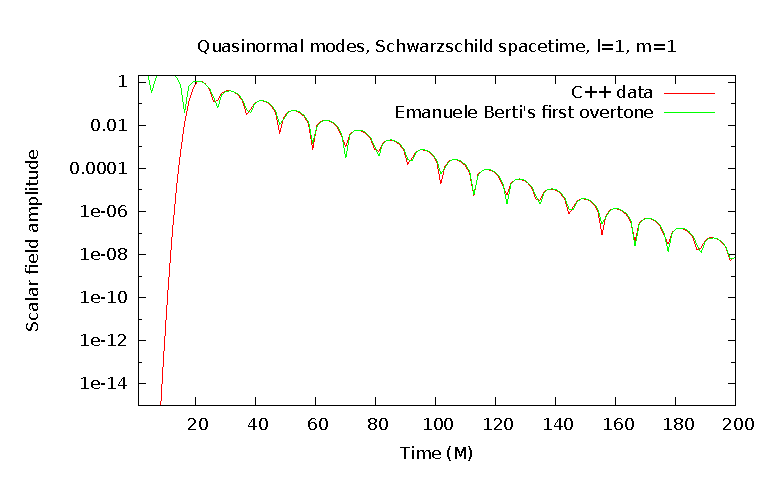
\includegraphics[width=\textwidth]{l1m1qnm}
      \caption{$l=1$}
    \end{subfigure}
    \begin{subfigure}{.45\textwidth}
      \centering
      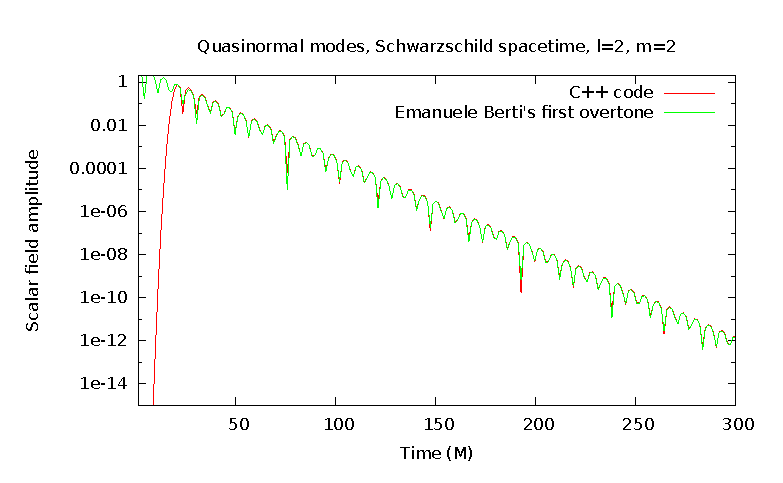
\includegraphics[width=\textwidth]{l2m2qnm}
      \caption{$l=2$}
    \end{subfigure}
  \caption{$l=2$ has a higher frequency and a faster decay rate than $l=1$}
  \end{figure}
\end{frame}

\begin{frame}
  \frametitle{Power law tails}
  \begin{figure}
    \centering
    \begin{subfigure}{.45\textwidth}
      \centering
      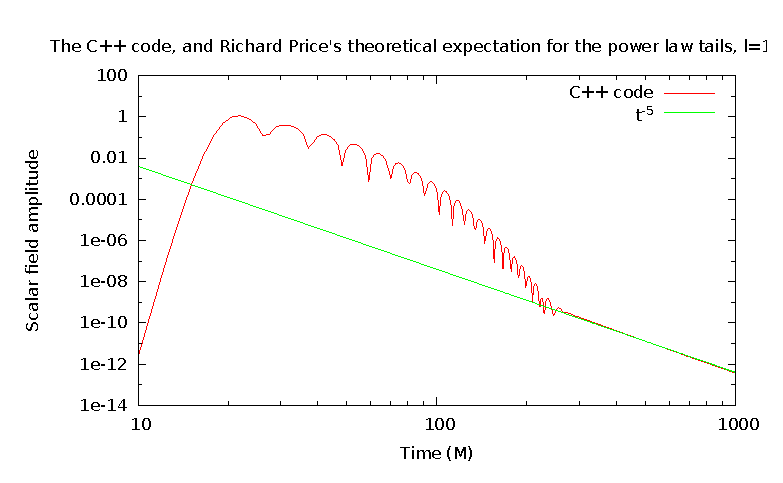
\includegraphics[width=\textwidth]{l1m1tail2}
      \caption{$l=1$}
  \end{subfigure}
    \begin{subfigure}{.45\textwidth}
      \centering
      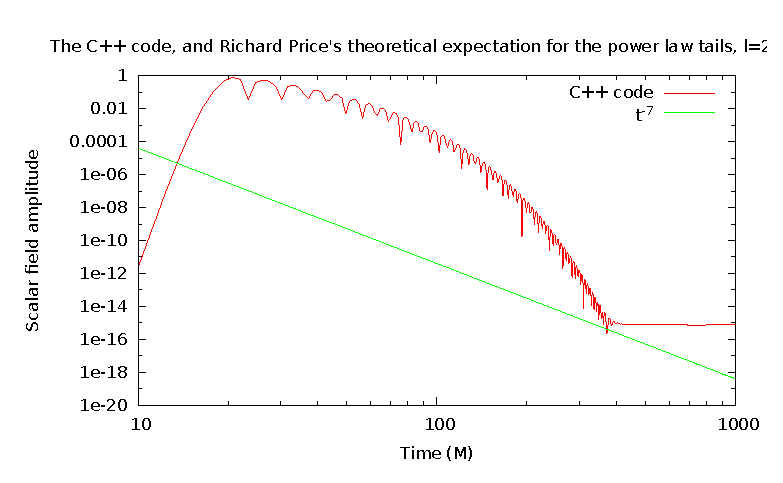
\includegraphics[width=\textwidth]{l2m2tailfail2}
      \caption{$l=2$}
    \end{subfigure}
  \caption{$l=1$ decays as $t^-{-5}$ as expected; however, $l=2$ has no power law tail due to truncation error}
  \end{figure}
\end{frame}



\begin{frame}
  \frametitle{The regular and singular field and effective source}
  \begin{itemize}
    \item Regularize field: $\Psi^R=\Psi^{ret}-\Psi^S$
  \item Detweiler-Whiting singular field: {\em Steven Detweiler, Bernard F. Whiting (2002). Phys. Rev. D 67, 024025}
  \item $\Box\Psi^R=S_{eff}=\Box\Psi^{ret}-\Box(W\tilde{\Psi}^S)$
  \item$\Box\Psi^{ret}=-4\pi q\int\delta_4(x,z(\tau^\prime))d\tau^\prime$
    \item In tensor case for gravitational field, perturbative expansion in terms of powers of radius
  \end{itemize}
\end{frame}

\begin{frame}
  \frametitle{Eccentric orbits using Peter Diener's simulation}
  \begin{itemize}
  \item $\chi$, $\phi$ $\rightarrow$ precession
  \item The orbit is artifically held on a geodesic to counteract the self-force generating the scalar waves
  \item $p$, $e$ held fixed, monotonically evolving $\chi$, $\phi$
  \item $r_{periastron}=\frac{pM}{1+e}$, $r_{apastron}=\frac{pM}{1-e}$
  \item Radial self-force: $F_r=q\partial_r\Psi^R$
  \end{itemize}
\end{frame}


\begin{frame}
  \frametitle{Self-force spherical harmonic components depend on time}
  \begin{figure}
    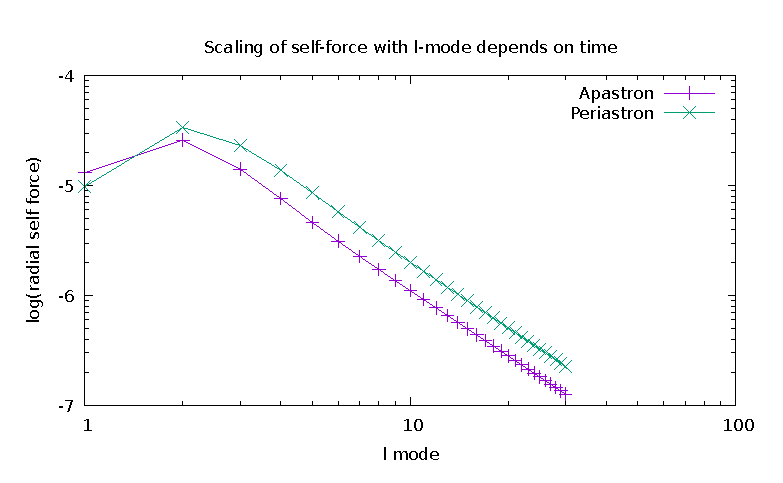
\includegraphics[width=0.9\textwidth]{lmodescalingdependsontime}
    \caption{Periastron has a higher self-force amplitude for nearly every spherical harmonic than apastron.}
  \end{figure}
\end{frame}

\begin{frame}
  \frametitle{The first order Richardson extrapolation}
  \begin{itemize}
  \item Discontinuous Galerkin: ODE solver with truncation errors that scale as $h^{n+1}$
  \item Assume $F_r(n,l)=F_{inf}(l)+c(l)\exp(-\alpha n)$
  \item Obtain extrapolation by solving system of equations for $F_r(n_i,l)$, $i=1,2,3$
   \end{itemize}
\end{frame}

\begin{frame}
  \frametitle{Well-converging data}
  \begin{figure}
  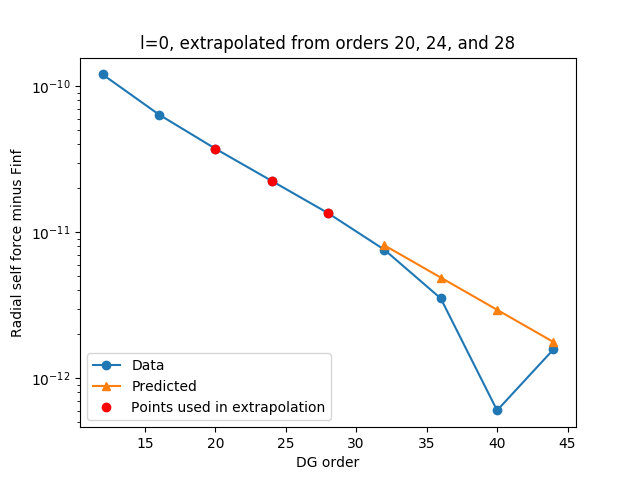
\includegraphics[width=0.9\textwidth]{fittingtechniqet370l0}
  \caption{l=0 at t=370. This data converges very cleanly until it hits roundoff noise at high DG orders.}
  \end{figure}
\end{frame}
  

\begin{frame}
  \frametitle{Error due to neglecting the first order Richardson extrapolation}
  \begin{figure}
    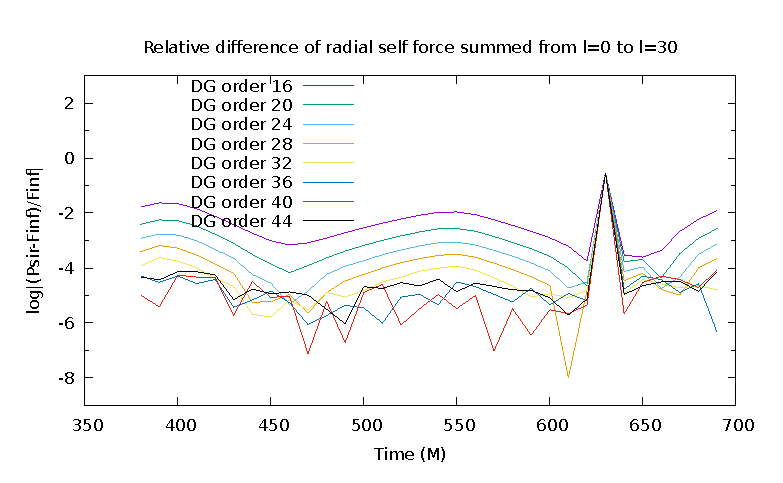
\includegraphics[width=0.9\textwidth]{reldiffpsirvtwfinfdgorders2}
    \caption{Relative error between DG starting orders and $F_{inf}$ vs time. For DG order 36 where roundoff error sets in, the error is about $10^{-4}$.}
  \end{figure}
\end{frame}

\begin{frame}
  \frametitle{The l-mode sum and fit}
  \begin{itemize}
  \item Use spherical harmonic decomposition of $\Psi$ to encode angular information
  \item must sum over $l$ and $m$ at end to obtain self force
  \item Use fit to extend sum to $l=\infty$
  \end{itemize}
  
  \begin{eqnarray}
    F_r(l,t)=&\frac{A(t)}{(2l-1)(21+3)}+\frac{B(t)}{(2l-3)(2l-1)(2l+3)(2l+5)}\nonumber \\
    &+\frac{C(t)}{(2l-5)(2l-3)(2l-1)(2l+3)(2l+5)(2l+7)}+\ldots
  \end{eqnarray}

   {\em Anna Heffernan, Adrian Ottewill, Barry Wardell (2012). Phys. Rev. D 86, 104023}

  \begin{itemize}
  \item Fit from $l_{min}$ to $l_{max}$.
  \item Sum numerically from zero to $l_{max}$ then use fit coefficients to analytically sum to $l=\infty$

  \end{itemize}
\end{frame}


\begin{frame}
  \frametitle{l-mode fit}
  \begin{figure}
    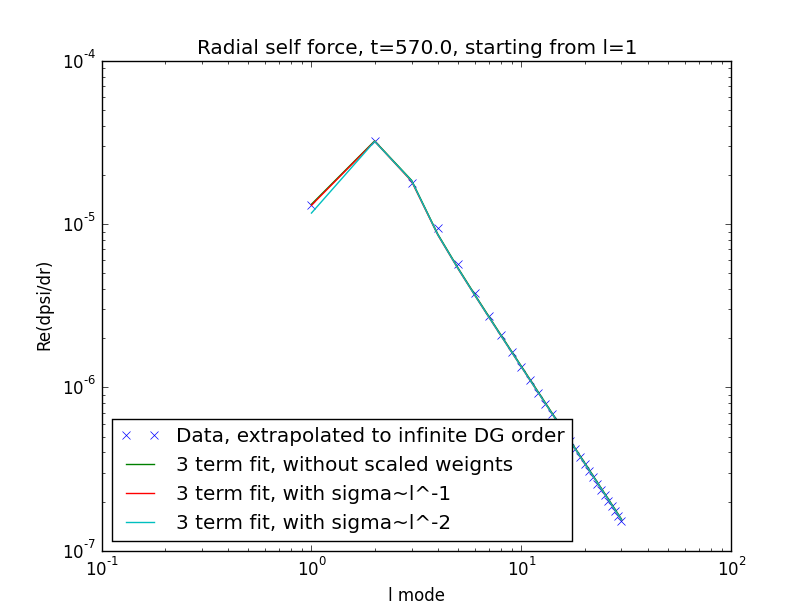
\includegraphics[width=0.9\textwidth]{fiterrscalecorrect3term570l1}
    \caption{l-mode versus $F_{inf}$.}
  \end{figure}
\end{frame}

\begin{frame}
  \frametitle{Smooth evolution of total radial self-force}
  \begin{figure}
    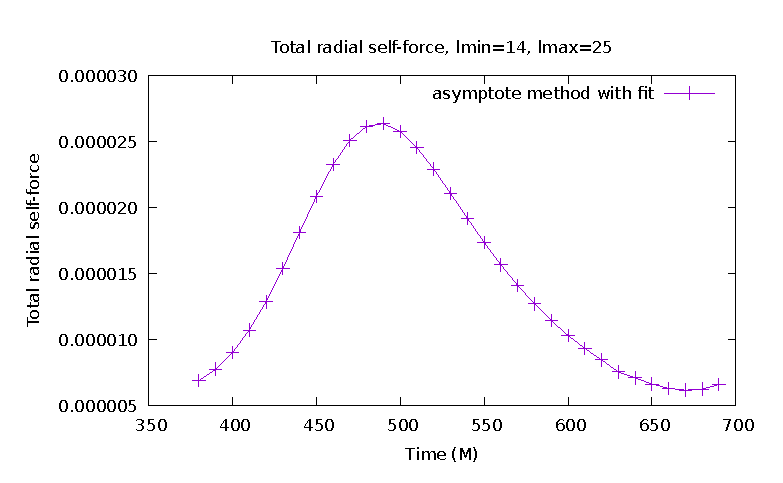
\includegraphics[width=0.9\textwidth]{totalselfforcevt2}
     \caption{Total radial self-force including sum to $l=\infty$ over time}
  \end{figure}
\end{frame}


\begin{frame}
  \frametitle{Error analysis conclusions}
  \begin{itemize}
  \item The relative error due to neglecting the first order Richardson extrapolation is $10^{-4}$. The best order at which to run is DG order 36. Limit dominated by roundoff error.
  \item The best $l_{min}=14$ and $l_{max}$=25. The relative error in these choice of values is $10^{-4}$.
  \item The relative error due to the number of terms used in the fit is $10^{-4}$.
  \item The error due to the use of weights in fitting is insignificant.
  \item These results are preliminary and need further investigation.    
  \end{itemize}
\end{frame}

      
\begin{frame}
  \frametitle{Comparison study of self-consistent to geodesic evolution}
  \begin{itemize}
  \item Self-consistent evolution naturally accounts for the interaction of the particle with the field it has generated in the past since it is evolved in the time domain
    \begin{itemize}
    \item The acceleration may need to be taken into account in the effective source
    \item The mass of the particle also evolves according to the work being done on it
    \item Evolved using the osculating orbits framework that slowly evolves $p$ and $e$ and has monetonic $\chi$ and $\phi$
    \item Capable of evolving to the plunge
    \end{itemize}
  \item Geodesic evolution uses a self-force that assumes the particle has been evolving on the same geodesic for all time
    \begin{itemize}
    \item Self-force can be efficiently calculated in the frequency domain due to periodicity
    \item Evolves in the time domain after generating the self-force in the frequency domain
    \item Cannot handle effects where the timescale of the orbital evolution is short compared to the period; therefore, cannot evolve to the plunge
    \end{itemize}
  \end{itemize}
\end{frame}

\begin{frame}
  \frametitle{Long term goals}
  \begin{itemize}
  \item Goal is to compare Diener's self-consistent code using Warburton's initial conditions and Wardell's effective source to Warburton's geodesic evolutions using frequency domain self force.
  \item I will run the simulation, examine physical quantities of interest, and help revise the simulation as necessary.
\item Specifically, it would be interesting to compare the rate of the phase evolution of the self force, since high precision in this quantity is required for LISA detections
  \item In particular, some instabilities in the self-consistent evolutions need to be addressed before a publication will be possible. I will help look for a solution to those instabilities. 
  \item Timescale: highly variable depending upon instabilities. 2-3 years potentially?
  \end{itemize}
\end{frame}

\begin{frame}
  \frametitle{Extra slides}
\end{frame}

\begin{frame}
  \frametitle{Flat space evolution}
  \begin{figure}
    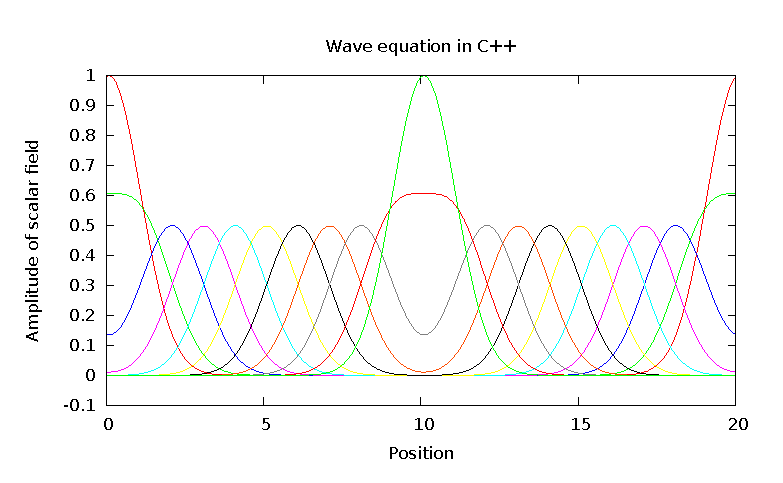
\includegraphics[width=4.0in]{gaussWave}
    \caption{Gaussian initial conditions, flat spacetime}
  \end{figure}
\end{frame}



\begin{frame}
  \frametitle{Flat spacetime error convergence}
  \begin{figure}
    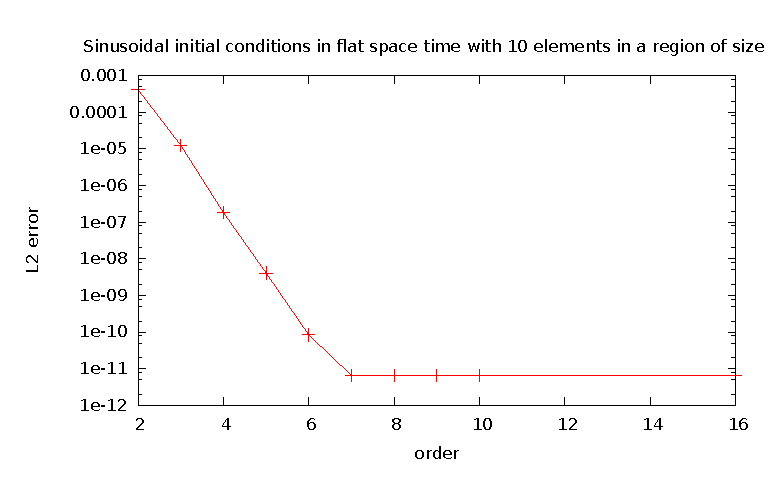
\includegraphics[width=4.0in]{sinL2WTorder}
    \caption{$L_2$ error converges exponentially until it hits roundoff noise with DG order for sinusiodal initial conditions with ten elements of size $h=0.01$.}
  \end{figure}
\end{frame}


\begin{frame}
  \frametitle{Circular orbit roundoff error comparison between languages}
  \begin{figure}
    \centering
    \begin{subfigure}{.45\textwidth}
      \centering
      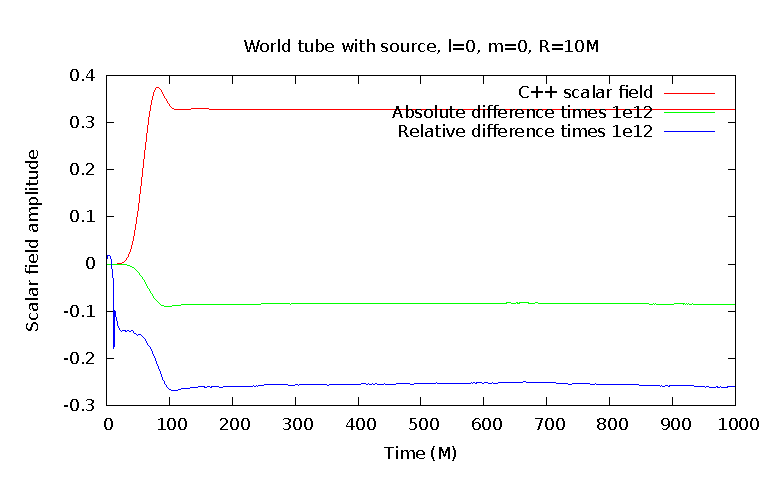
\includegraphics[width=\textwidth]{wtcircl0m0}
      \caption{l=0}
   \end{subfigure}
    \begin{subfigure}{.45\textwidth}
      \centering
      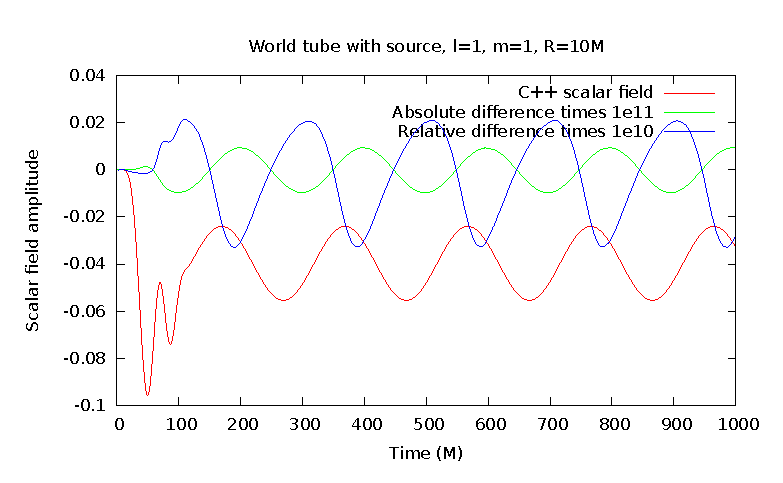
\includegraphics[width=\textwidth]{wtcircl1m1}
      \caption{l=1}
    \end{subfigure}
  \caption{Relative and absolute errors are at the roundoff level-- $10^{-10}$ to $10^{-12}$. Oscillations do not appear in the $l=0$ mode but appear with the orbital period in the $l=1$ mode.}
  \end{figure}
\end{frame}

\begin{frame}
  \frametitle{Precession of the eccentric orbit}
  \begin{figure}
    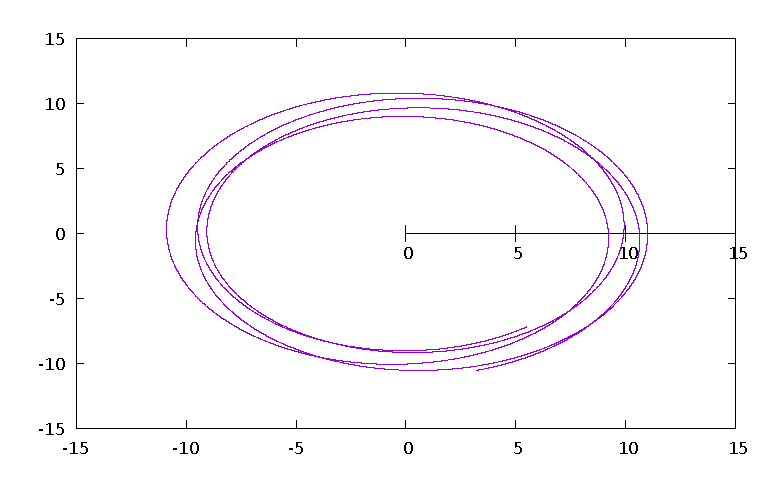
\includegraphics[width=0.9\textwidth]{orbitevolvedg44p99e01}
    \caption{Precession of the eccentric orbit. $p=9.9$, $e=0.0$.}
  \end{figure}
\end{frame}

\begin{frame}
  \frametitle{Evolution of the radial self-force for different initial conditions}
  \begin{figure}
  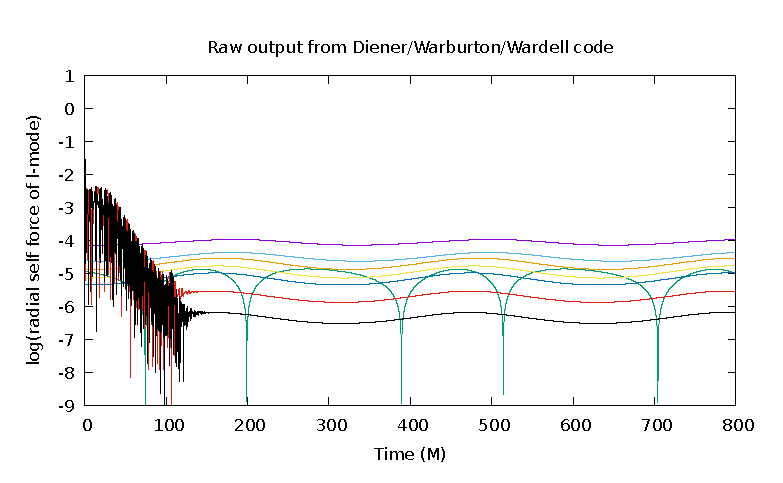
\includegraphics[width=0.9\textwidth]{rawRadialSelForceModes}
  \caption{Low $l$ behavior of the self-force for a given l-mode summed over $m$}
  \end{figure}
\end{frame}


\begin{frame}
  \frametitle{Residuals to the l-mode fit}
  \begin{figure}
    \centering
    \begin{subfigure}{.45\textwidth}
      \centering
      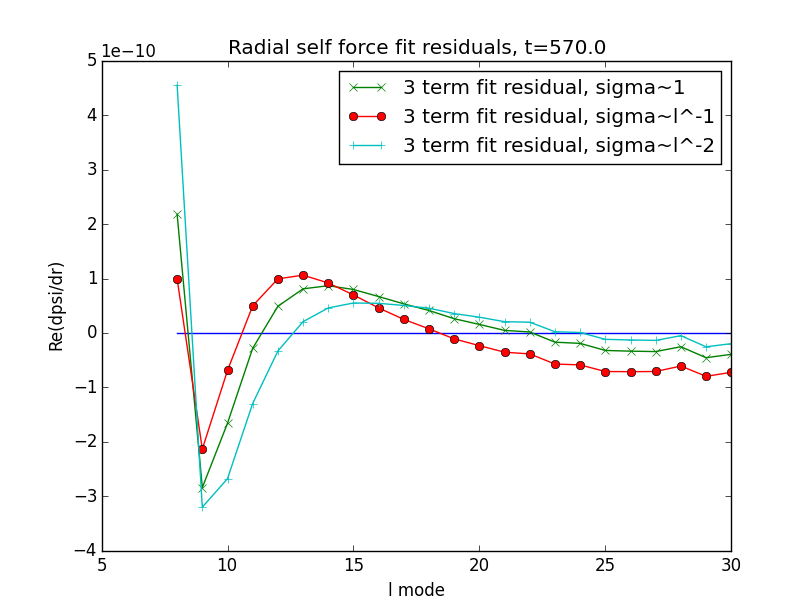
\includegraphics[width=\textwidth]{fitresiduals3terms570l8}
      \caption{$l_{min}=8$}
    \end{subfigure}
    \begin{subfigure}{.45\textwidth}
      \centering
      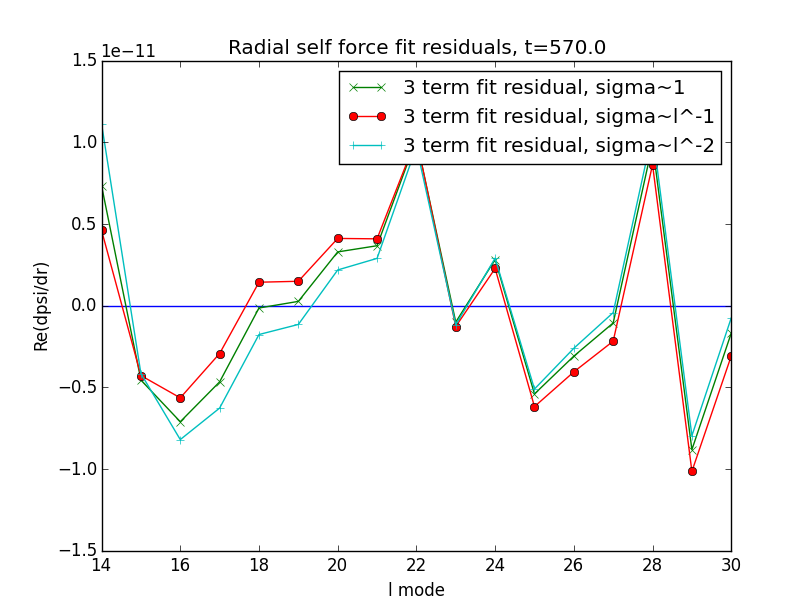
\includegraphics[width=\textwidth]{fitresidulas3terms570l14}
      \caption{$l_{min}=14$}
    \end{subfigure}
  \caption{$l_{min}=14$ is a better fit than $l_{min}=8$ both because it is less systematically biased and because it has an amplitude an order of magnitude smaller. Both fits end at $l_{max}=30$.}
  \end{figure}
\end{frame}

\begin{frame}
  \frametitle{Roundoff noise in $F_{inf}$ at high $l_{max}$}
  \begin{figure}
    \centering
    \begin{subfigure}{.45\textwidth}
      \centering
      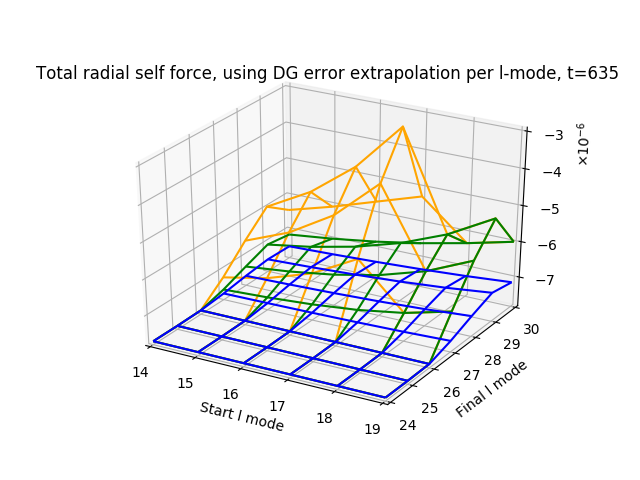
\includegraphics[width=\textwidth]{bestfinflminlmax234terms635fullrange_perihelion}
      \caption{Large range}
    \end{subfigure}
    \begin{subfigure}{.45\textwidth}
      \centering
      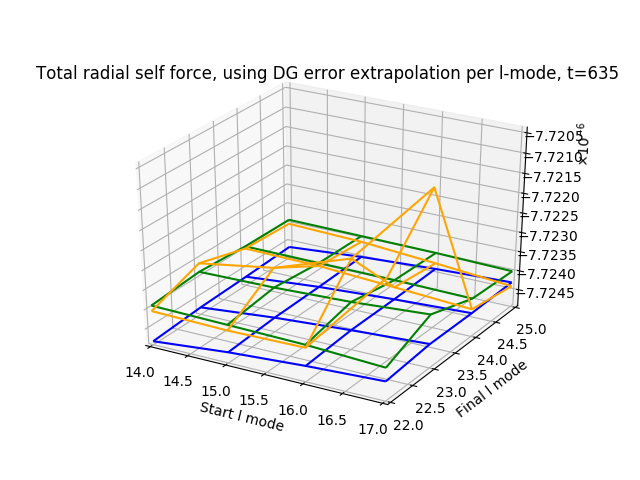
\includegraphics[width=\textwidth]{bestfinflminlmax234termst635smallrange_perihelion}
      \caption{Small range}
    \end{subfigure}
  \caption{$l_{min}=14$ and $l_{max}=25$ appear to be good start and stop values. Roundoff noise is evident at higher l.}
  \end{figure}
\end{frame}


\begin{frame}
  \frametitle{Error due to l-mode selection, number of terms}
  \begin{figure}
    \centering
    \begin{subfigure}{.45\textwidth}
      \centering
      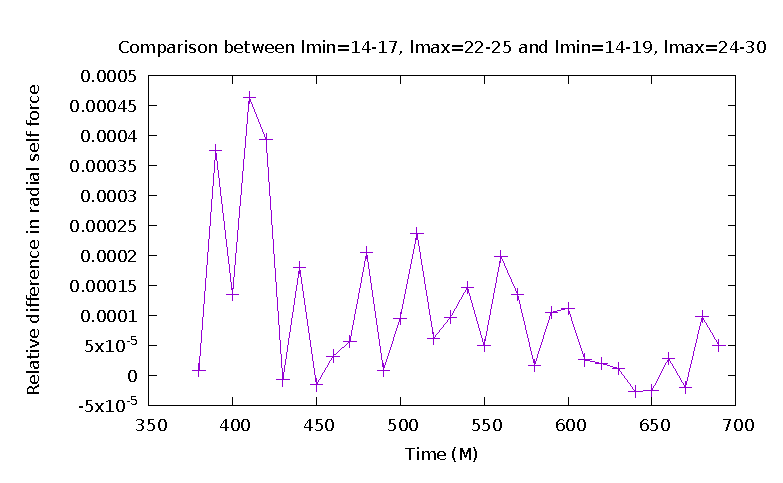
\includegraphics[width=\textwidth]{relErrBigSmallRangeOverTime}
      \caption{large versus small range}
    \end{subfigure}
    \begin{subfigure}{.45\textwidth}
      \centering
      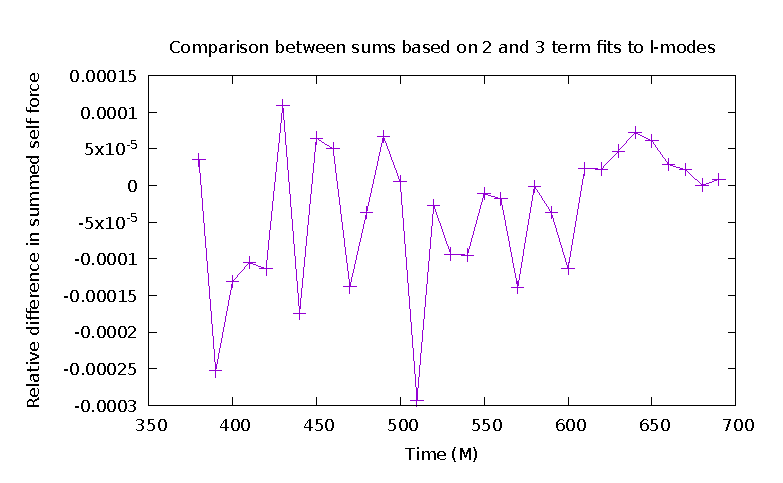
\includegraphics[width=\textwidth]{relativeError23termSelfForce}
      \caption{2 versus 3 terms}
    \end{subfigure}
  \caption{Relative errors in both of these effects appear to be at the $10^{-4}$ level.}
  \end{figure}
\end{frame}


\end{document}
